\documentclass[a4paper, 11pt]{report}

\usepackage[utf8]{inputenc} % Définit l'encodage du document
\usepackage[T1]{fontenc} % Définit l'encodage de la fonte
\usepackage[francais]{babel} % Spécifie que le document est en français
\usepackage{graphicx}
\graphicspath{{.}}

\usepackage{lipsum}

\begin{document}
        \title{BE 3 - Extraction de connaissances}
        \author{Jordan \bsc{Abderrachid}\\ Thomas \bsc{Perrot}\\ Louis \bsc{Zawadski}}

        \maketitle

\section{Exercice I}

        On applique l'algorithme \emph{FarthestFirst} à la base de données \emph{weather.arff}. On obtient les résultats présentés dans le tableau ci-dessous.
	\begin{table}[h!]
	\centering
	\begin{tabular}{|c|c|c|c|c|c|}
		\hline
		Cluster & Outlook & Température & Humidity & Windy & Play \\
		\hline
		Cluster0 : & overcast & 72.0 & 90.0 & TRUE & yes \\
		\hline
		Cluster1 : & sunny & 85.0 & 85.0 & FALSE & no \\
		\hline
	\end{tabular}
	\caption{Centroïdes calculés par l'algorithme \emph{FarthestFirst} avec 2 clusters}
	\label{exo1}
\end{table}

        \section{Exercice II}
        On applique l'algorithme \emph{SimpleKMeans} à la base de données \emph{weather.arff}. On obtient les résultats présentés dans le tableau ci-dessous.
        
        \begin{table}[h!]
        \centering
        \begin{tabular}{| l | l | l | l | l | l |}
        \hline
        Cluster & Outlook & Temperature & Humidity & Windy & Play \\
        \hline
        Cluster 0 & sunny & 75.9 & 84.1 & FALSE & yes \\
        \hline
        Cluster 1 & overcast & 69.4 & 77.2 & TRUE & yes \\
        \hline

        \end{tabular}
        \caption{Centroïdes calculés par l'algorithme \emph{SimpleKMeans} avec 2 clusters}
        \label{tab:exo_2}
        \end{table}
        
        \section{Exercice III}
        On peut remarquer que les centroïdes des clusters sont beaucoup plus proches dans le cas de \emph{SimpleKMeans}. Par ailleurs, l'algorithme Fartherst-First génère un cluster correspondant à Play=no et un autre à Play=yes. On peut donc en déduire que l'algorithme qui maximise le plus la dispersion inter-cluster est l'algorithme Farthest-First.
        
	\section{Exercice V}
	On applique les successivement les algorithmes \emph{FarthestFirst } et \emph{SimpleKMeans} à la base de données \emph{weather.arff} en chochant l'option "Store clusters for visualization". On obtient les résultats présentés dans le tableau ci-dessous.

	\begin{table}[h!]
		\centering
		\begin{tabular}{|l|c|l|c|}
			\hline
			Outlook : & overcast  & Outlook : & rainy \\
			Windy : & TRUE & Windy : & TRUE \\
			\hline
			Outlook : & overcast & Outlook : & rainy \\
			Windy : & FALSE & Windy : & FALSE \\
			\hline
		\end{tabular}
		\caption{Combinaisons de valeurs de outlook et windy pour lesquelles toutes les instances appartiennent au cluster 0 pour la méthode \emph{FarthestFirst}.}
		\label{tab:exo5-1}
	\end{table}


	\begin{table}[h!]
		\centering
		\begin{tabular}{|l|c|l|c|}
			\hline
			Outlook : & sunny & Outlook : & X \\
			Windy : & FALSE & Windy : & X \\
			\hline
		\end{tabular}
		\caption{Combinaisons de valeurs de outlook et windy pour lesquelles toutes les instances appartiennent au cluster 1 pour la méthode \emph{FarthestFirst}.}
		\label{tab:exo5-1}
	\end{table}

        \section{Exercice VI}
        On change le paramètre seed de l'algorithme \emph{SimpleKMeans}. On remarque que les clusters sont initialisés avec play=yes pour l'un et play=no pour l'autre.
        \begin{table}[h!]
        \centering
        \begin{tabular}{| l | l | l | l | l | l |}
        \hline
        Cluster & Outlook & Temperature & Humidity & Windy & Play \\
        \hline
        Cluster 0 & sunny & 75 & 84.1 & FALSE & yes \\
        \hline
        Cluster 1 & sunny & 71 & 77.2 & TRUE & no \\
        \hline

        \end{tabular}
        \caption{Centroïdes calculés par l'algorithme \emph{SimpleKMeans} avec un seed différent}
        \label{tab:exo_6}
        \end{table}
        
        \section{Exercice VII}
        On visualise les résultats obtenus par la simulation précédente. On remarque que les combinaisons de valeurs suivantes appartiennent au cluster 0 :
        \begin{table}[h!]
        \centering
        \begin{tabular}{| c | c |}
         \hline
         Outlook & Windy \\
         \hline
         sunny & false \\
         overcast & false \\
         rainy & false \\
         \hline
        
        \end{tabular}
        \caption{Couples Outlook-Windy appartenant au cluster 0}
        \label{tab:exo7_1}
        \end{table}
        
        Les couples suivants appartiennent au cluster 1 : 
        \begin{table}[h!]
        \centering
        \begin{tabular}{| c | c |}
         \hline
         Outlook & Windy \\
         \hline
         sunny & true \\
         rainy & true \\
         \hline
        
        \end{tabular}
        \caption{Couples Outlook-Windy appartenant au cluster 1}
        \label{tab:exo7_2}
        \end{table}

        \section{Exercice VIII}
        On compare les résultats obtenus avec \emph{Farthest-First} et \emph{SimpleKMeans}. On peut remarquer que les couples de valeurs outlook-windy suivantes ont des clusters différents selon la classification : 
        \begin{table}[h!]
        \centering
        \begin{tabular}{| c | c |}
         \hline
         Outlook & Windy \\
         \hline
         sunny & false \\
         overcast & true \\
         rainy & true\\
         \hline
        
        \end{tabular}
        \caption{Couples Outlook-Windy ayant des clusters différents}
        \label{tab:exo8}
        \end{table}
        
        \section{Exercice IX}
        On affiche côte-à-côte les graphiques représentant l'appartenance au cluster et l'attribut play pour les couples de valeurs Outlook-Windy.
        On remarque des différences pour les couples de valeur suivants :
        \begin{table}[h!]
        \centering
        \begin{tabular}{| c | c |}
         \hline
         Outlook & Windy \\
         \hline
         sunny & false \\
         sunny & true \\
         \hline
        
        \end{tabular}
        \caption{Couples Outlook-Windy ayant des valeurs de play et des clusters différents}
        \label{tab:exo9}
        \end{table}
        

	\section{Exercice X}
	On execute les algorithmes \emph{FarthestFirst} et \emph{SimpleKMeans} en utilisant l'option Classes to clusters evaluation et en sélectionnant l'attribut play comme attribut de classe. Les résultats sont visibles sur le figure ci-dessous.

	\begin{table}[h!]
		\centering
		\begin{tabular}{|c|c|c|}
			\hline
			Valeur / Méthode & \emph{FarthestFirst} & \emph{SimpleKMeans} \\
			\hline
			Nb. faux Positifs & 3 & 2 \\
			\hline
			Nb. faux Négatifs & 6 & 3 \\
			\hline
			Taux d'erreur & 35.7\% & 35.7\% \\
			\hline
		\end{tabular}
		\caption{Comparaison de \emph{FarthestFirst} et \emph{SimpleKMeans} avec l'option Classes to Clusters evaluation avec play comme attribut de classe.}
		\label{tab:exo10}
	\end{table}

	\section{Exercice XI}
	On cherche le seed qui minimuse les erreurs commises par les algorithmes \emph{FarthestFirst} et \emph{SimpleKmeans} avec l'option Classes to clusters evaluation et en sélectionnant l'attribut play comme attribut de classe. On test pour seed valant 1, 10, 20, 50, 100 et 1000. Les meilleurs résultats sont consignés dans le tableau ci-dessous.

	\begin{table}[h!]
		\centering
		\begin{tabular}{|c|c|c|c|c|}
			\hline
			SimpleKMeans & Seed & Taux d'err & Play=yes mal placées & Play=no mal placées \\
			\hline
			\emph{SimpleKMeans} & 100 & 28.6\% & 3 & 1 \\
			\hline
			\emph{FarthestFirst} & 1 & 35.7\% & 6 & 1 \\
			\hline
		\end{tabular}
		\caption{Détermination de la meilleure valeur de seed pour les méthodes \emph{SimpleKMeans} et \emph{FarthestFirst}}
		\label{tab:exo11}
	\end{table}

	\paragraph{Conclusion}Au vu des résultats précédents, l'algorithme qui génère le moins grand nombre d'erreurs est \emph{SimpleKMeans}.

	\section{Exercice XII}
	On visualise le meilleur résultat de l'exercice précédent, et on reporte dans un tableau ci-dessous les combinaisons de valeurs de outlook et windy pour lesquelles aucune erreur n'est commise.

	\begin{table}[h!]
		\centering
		\begin{tabular}{|l|c|l|c|}
			\hline
			Outlook : & overcast  & Outlook : & rainy \\
			Windy : & FALSE & Windy : & FALSE \\
			\hline
			Outlook : & sunny & Outlook : & X \\
			Windy : & FALSE & Windy : & X \\
			\hline
		\end{tabular}
		\caption{Combinaisons de valeurs de outlook et windy pour lesquelles aucune erreur n'est commise avec la méthode \emph{FarthestFirst} et seed=100.}
		\label{tab:exo12}
	\end{table}

        \section{Exercice XIII}
        	On applique l'algorithme de \emph{clustering} \texttt{DBScan} à notre base de donnée, en faisant varier le nombre minimum de points par \emph{cluster}. On conserve le meilleur résultat.

    	\begin{table}[h!]
    		\centering
    		\begin{tabular}{|c|c|c|c|c|}
    		\hline
    		Algo & MinPoints & Taux d'err & Play=yes mal placés & Play=no mal placés \\
    		\hline
    		\texttt{DBScan} & 3 & 28,57\% & 2 & 2\\
    		\hline
    		\end{tabular}
    		\caption{Résultats de la méthode \texttt{DBScan} optimisant le nombre minimum de points par \emph{cluster}.}
        	\label{tab:exo13}
    	\end{table}



    	\section{Exercice XIV}
    		On applique l'algorithme de \emph{clustering} \texttt{DBScan} à notre base de donnée, en faisaint varier la valeur de $\epsilon$, c'est à dire le rayon de chaque \emph{cluster}. On fixe le nombre minimum de points par cluster à 2. On conserve le meilleur résultat.

		\begin{table}[h!]
			\centering
			\begin{tabular}{|c|c|c|c|c|}
				\hline
				Algo & $\epsilon$ & Taux d'err & Play=yes mal placés & Play=no mal placés \\
				\hline
				\texttt{DBScan} & 1,04 & 35,71\% & 1 & 4 \\
				\hline
			\end{tabular}
			\caption{Résultats de la méthode \texttt{DBScan} optimisant le rayon de chaque \emph{cluster}.}
        	\label{tab:exo14}
		\end{table}

      \section{Exercice XVI}
        On effectue l'algorithme EM pour différentes valeurs de seed. On obtient les mêmes résultats pour toutes les valeurs de seed de 1 à 1000, à savoir celle présentée dans le tableau ci-dessous : 
        \begin{table}[h!]
        \centering
        \begin{tabular}{| c | c | c | c | c |}
        \hline
         Algo & Seed & Taux d'erreur & Faux négatifs & Faux positifs  \\
         \hline
         EM & x & 35\% & 2 & 3 \\
         \hline
         
        \end{tabular}
        \caption{Résultats de l'algorithme EM}
        \label{tab:exo16}
        \end{table}
        
        \section{Exercice XVII}
        On peut relever les valeurs les plus probables dans les clusters générés par la méthode EM :
        \begin{table}[h!]
        \centering
        \begin{tabular}{| l | l | l | l | l | l |}
        \hline
        Cluster & Outlook & Temperature & Humidity & Windy & Play \\
        \hline
        Cluster 0 & rainy & 70.2 & 80.7 & TRUE & yes \\
        \hline
        Cluster 1 & overcast & 82.2 & 84.0 & FALSE & no \\
        \hline

        \end{tabular}
        \caption{Valeurs les plus probables dans les clusters EM}
        \label{tab:exo_6}
        \end{table}
        
        \section{Exercice XVIII}
        On teste l'algorithme Cobweb avec différentes valeurs pour le \emph{CutOff}. On remarque que l'on obtient 2 clusters pour un \emph{CutOff} de 0,24. On obtient le résultat suivant : 
        
        \begin{table}[h!]
        \centering
        \begin{tabular}{| c | c | c | c | c |}
        \hline
         Algo & CutOff & Taux d'erreur & Faux négatifs & Faux positifs  \\
         \hline
         Cobweb & 0.24 & 35\% & 3 & 2 \\
         \hline
         
         
        \end{tabular}
        \caption{Résultats de l'algorithme Cobweb}
        \label{tab:exo18}
        \end{table}

        \section{Exercice XX (Bonus)}
        On applique les algorithmes \emph{Cobweb} et \emph{EM} à la base de données titanic.arff. On obtient les résultats suivants :
        \begin{table}[h!]
        \centering
        \begin{tabular}{| c | c | c | c | c |}
        \hline
         Algo & CutOff/Seed & Taux d'erreur & Faux négatifs & Faux positifs  \\
         \hline
         Cobweb & 0.175 & 22\% & 367 & 126 \\
         \hline
         EM & 10 & 46\% & 212 & 817 \\
         \hline
         
        \end{tabular}
        \caption{Comparaison Cobweb et EM sur la base titanic}
        \label{tab:exo20}
        \end{table}
        
        On peut déduire de ces résultats que l'algorithme Cobweb sont meilleurs que celui de l'algorithme EM.
        

	\section{Exercice XXI}
	On étudie les 6 clusters issus de la base de données Bank-data.csv. En analysant la proximité de chaque cluster avec les autres, on reporte dans un tableau le nombre de paramêtres similaires entre les différents clusters. Le résultat est visible dans le tableau ci-dessous. On regroupe alors les clusters en utilisant une méthode de clustering agglomérative. On trouve ainsi une proximitée très forte entre les clusters 1 et 2 (nouveau cluster $C_{1,2}$), puis 3 et 4 (nouveau cluster $C_{3,4}$), puis 3 et 5 (nouveau cluster $C_{3,4,5}$), puis 2 et 3 (nouveau cluster $C_{1,2,3,4,5}$). On a donc 2 clusters : $C_{1,2,3,4,5}$ et $C_6$.
	
	\begin{table}[h!]
\centering
\begin{tabular}{| c | c | c | c | c | c | c |}
\hline
Cluster & 1 & 2 & 3 & 4 & 5 & 6 \\
\hline
1 & 0 & 8 & 4 & 5 & 1 & 4 \\
\hline
2 & & 0 & 7 & 6 & 5 & 3 \\
\hline
3 & & & 0 & 8 & 7 & 3 \\
\hline
4 & & & & 0 & 4 & 3 \\
\hline
5 & & & & & 0 & 5 \\
\hline

\end{tabular}
\caption{Nombre d'attributs proches entre clusters}
\label{tab:exo20}
\end{table}

	\section{Exercice XXII}
	Lorsque nous avons regroupé les clusters dans la question précédente, nous avons regardé des attibuts booléens. Ainsi, nous avons toujours considéré qu'un YES est plus proche d'un YES que d'un NO par exemple. Or, lorsqu'on regarde les pourcentage, on s'apperçoit que deux clusters qui semblaient séparés (l'un a l'attribut à YES, l'autre à NO) peuvent être proches en terme de pourcentage (voire être plus proches en pourcentage que deux YES ou deux NO). Il est donc important de regarder les pourcentages et pas seulement les résultats booléens lorsqu'on veut faire du clustering.

	\section{Exercice XXIII}
	En choississant deux clusters dans les options de Weka, on obtient au final deux clusters contenant respectivement 247 (41\%) et 353 (59\%) instances. Il semble que les attributs numériques ne sont pas pris en compte, car ceux-ci sont très proches dans les deux clusters. Les deux clusters se distinguent sur les attributs à deux valeurs suivants : "sex", "married" et "pep", les autres attributs sont similaires. Ces résultats diffèrent de ceux que nous avions trouvé, ce qui est normal dans la mesure où nous avions pris en compte les valeurs numériques dans nos calculs de distances.

   
        \section{Exercice XXIV}
        On applique K-means ++ à la base de données bank-data. On observerve les meilleurs résultats pour $seed = 10$. Pour cette valeur de seed on obtient les résultats suivants sur les 60 instances de test :
        
        \begin{table}[h!]
        \centering
        \begin{tabular}{| c | c | c | c | c |}
        \hline
         Algo & Seed & Taux d'erreur & Faux négatifs & Faux positifs  \\
         \hline
         K-means++ & 10 & 16\% & 4 & 6 \\
         \hline
        \end{tabular}
        \caption{Application de k-means ++}
        \label{tab:exo24}
        \end{table}
        
        \section{Exercice XXV}
        On applique la méthode de classification J48 à l'ensemble de test en demandant de déterminer le cluster. On parvient à classer correctement toutes les instances grâce aux règles suivantes : 
        \begin{table}[h!]
        \centering
        \begin{tabular}{l l l l}
        Si pep=YES & & & \\
         // & Si sex = FEMALE & & \\
         // & // & Si car = NO & alors cluster NO \\
         // & // & Si car = YES & alors cluster YES \\
         // & Si sex = MALE & & alors cluster YES \\
        Si pep = NO & & & \\
         // & Si car = NO & & alors cluster NO \\
         // & Si car = YES & & \\
         // & // & Si sex = FEMALE & alors cluster NO \\
         // & // & Si sex = MALE & alors cluster YES\\
        \end{tabular}
        \caption{Règles de classification de l'ensemble de test clusterisé}
        \label{tab:exo25}
        \end{table}
        
        \section{Exercice XXVI}
        On applique K-means ++ à l'ensemble des instances de la base de données bank-data.
        On obtient le meilleur résultat pour un seed de 52. On obtient alors les valeurs suivantes :
        \begin{table}[h!]
        \centering
        \begin{tabular}{| c | c | c | c | c |}
        \hline
         Algo & Seed & Taux d'erreur & Faux négatifs & Faux positifs  \\
         \hline
         K-means++ & 52 & 42\% & 145 & 108 \\
         \hline
        \end{tabular}
        \caption{Application de k-means ++}
        \label{tab:exo26}
        \end{table}
        
        On remarque que cette méthode de clustering n'est pas très efficace.
        
        
        \section{Exercice XXVII}
        On applique la méthode de classification J48 à la base de données ainsi clusterisée. On obtient les règles suivantes :
        \begin{figure}[h!]
        \centering
        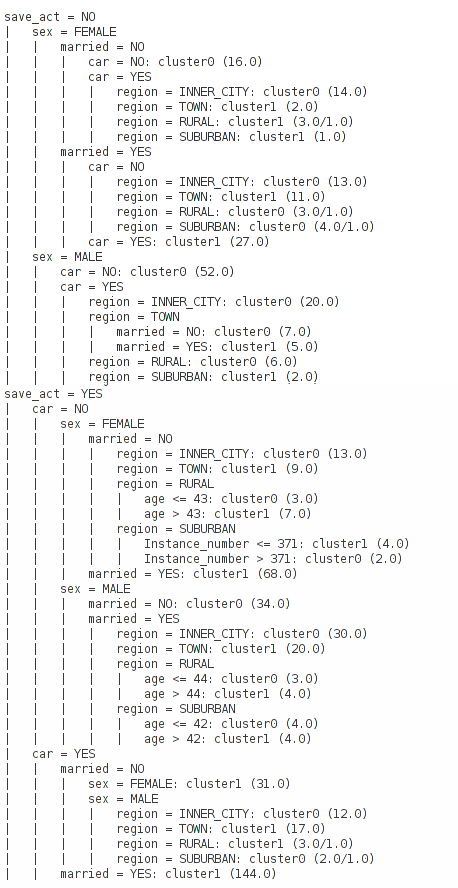
\includegraphics[scale=0.4]{regles27}
        \caption{Règles de classification}
        \label{fig:exo27}
        \end{figure}

        \section{Exercice XXVIII}
        On applique la méthode EM (Expectation-Maximisation) à la base de données bank-data avec les paramètres par défaut.
        
        On obtient les résultats suivants :
        \begin{table}[h!]
        \centering
        \begin{tabular}{| c | c | c | c | c |}
        \hline
         Algo & Seed & nb plis & clusters & log-vraisemblance  \\
         \hline
         EM & 100 & 10 & 4 & -20,9 \\
         \hline
        \end{tabular}
        \caption{Application de l'algorithme EM}
        \label{tab:exo28}
        \end{table}
        
        On fait varier les différents paramètres.
        
        Le meilleur résultat est obtenu pour un seed de 50. On obtient alors le résultat suivant pour 10 plis :
        \begin{table}[h!]
        \centering
        \begin{tabular}{| c | c | c | c | c |}
        \hline
         Algo & Seed & nb plis & clusters & log-vraisemblance  \\
         \hline
         EM & 50 & 10 & 5 & -18,5 \\
         \hline
        \end{tabular}
        \caption{Meilleur résultat de l'algorithme EM}
        \label{tab:exo282}
        \end{table}
        
        \section{Exercice XXIX}
        On active l'évaluation des clusters par l'appartenance à une classe. On remarque que ce mode associe un cluster à chacune des classes. Sachant qu'on chercher à mesurer l'efficacité des clusters par rapport à un variable pouvant appartenir à 2 classes différentes, on obtient le meilleur résultat lorsque l'on se limite à deux clusters, dans ce cas on peut arriver à classer correctement 58\% des instances, ce qui est très faible. 
        
        Suite à l'utilisation de l'algorithme EM, nous pouvons dire qu'il est peu aisé de régler celui-ci correctement, de plus la durée de l'apprentissage étant relativement longue sur nos machines (entre 20 et 30 secondes), tester les différents paramètres de la simulation peut prendre un temps considérable.
        
        \section{Exercice  XXX}
        On choisit cette fois-ci la méthode MakeDensityBasedClusterer, que l'on applique successivement à Canopy, Cobweb, Hierarchical, EM et SimpleKMeans. On applique ces méthodes sur les données d'apprentissage Bank-data. On peut alors comparer la log-vraisemblance que l'on obtient :
        
        \begin{table}[h!]
        \centering
        \begin{tabular}{| c | c |}
        \hline
         Algo & log-vraisemblance  \\
         \hline
         Canopy & -22,12 \\
         \hline
         Cobweb & -22,04 \\
         \hline
         Hierarchichal & -22,09\\
         \hline
         EM & -21,65\\
         \hline
         SimpleKMeans & -22,18\\
         \hline
        \end{tabular}
        \caption{Résultat pour le clusterer à base de densité}
        \label{tab:exo30}
        \end{table}
        
        On peut remarquer que les méthodes ont des logs-vraisemblance assez proche, et en cherchant à optimiser leur paramètres on pourrait probablement arriver à un classement différent.

\end{document}
